\section{Introduction}

% Do we have any more papers that we can cite around the role of colorization in helping people read formulas?
% Our current strongest argument is that authors are already doing this; though it would be even stronger if we could write that people *should be* doing this.

% Motivation we could draw on from the literature is:
% * Preattentive features help people rapidly find features of interest in complex visuals---this likely applies to helping people find corresponding expressions in a formula that relate to descriptive text.
% * Color and labels serve as a mechanism for linking across registers.
% * Our perceptual systems are retrained to parse mathematics, and perhaps one role of colors and annotations is to provide scaffolding for people to recognize important structures in math formulas [Marghetis et al. 2016]
% (Andrew continue from here)

% We probably don't want to lead with data science and machine learning
% These challenges are pervasive across fields---data science and machine learning are one example
% Can we start with an example. Imagine you are a student in such a class. Start out with a scenario (a specific formula), describe the difficulties that people face.
% Can the introduction describe the value in a more visceral way.
% Then we can ground it in principles as to why this presentation might improve the reading of the formula.
% Improve Gestalt of the teaser figure
% Nota, Heardown---if we include, cite it much earlier on as parenthetical of prior work.
% drop "sufficient practice"---it is 

% \andrew{Danaë's most ambitious suggestion, which I think we should try, is to try to make the value of augmentation more visceral in the introduction. Could we show a formula that would be difficult to understand on its own, and then show it augmented a few sentences later, as an opportunity to provide a clearer indication of why it is useful to augment a formula? To pilot this idea, we could try to take the formula from the demo, and show it without and then with labels.}

% \andrew{See Danaë's other suggestions as margin comments in Overleaf.}

Notation poses a barrier to understanding mathematical ideas. Whether in the physics classroom, data science research papers~\cite{ref:mysore2023how}, or programming documentation~\cite{ref:cai2019software}, readers find important knowledge locked behind the formalisms of formulas and symbols. 
% The complexities of mathematical notation (e.g., unfamiliar symbols, domain-specific conventions) pose a barrier to those seeking to understand powerful mathematical ideas in the languages that they are expressed. As a result, many learners find themselves stymied in understanding learning resources that make use of notation—especially when the background of the reader does not match the expectations of the learning material~\cite{ref:cai2019software,ref:mysore2023how}.
Consider a reader encountering this formula in a research paper \cite{ref:hohman2019gamut}:

% To develop this understanding, learners need to engage with mathematical ideas in the languages that they are expressed. However, when the background of the reader does not match the expectations of the learning material, this could impose a barrier to effective comprehension.

\begin{center}
\vspace{1ex}

\includegraphics[width=0.62\linewidth]{figures/pre-aug-intro}
\end{center}
\vspace{-0.5ex}

This formula represents a linear regression model. If the reader is not familiar with its idioms, they are likely to find it hard to understand. For instance, what is ``$x$'' and how is it different from ``$\beta$''? $\beta_0$ and $\beta_1$ share a common base---how are they related? What is the intuition of the formula as a whole?

Suppose the formula was instead shown as follows:

% \vspace{-.2ex}
\begin{center}
\vspace{0.5ex}
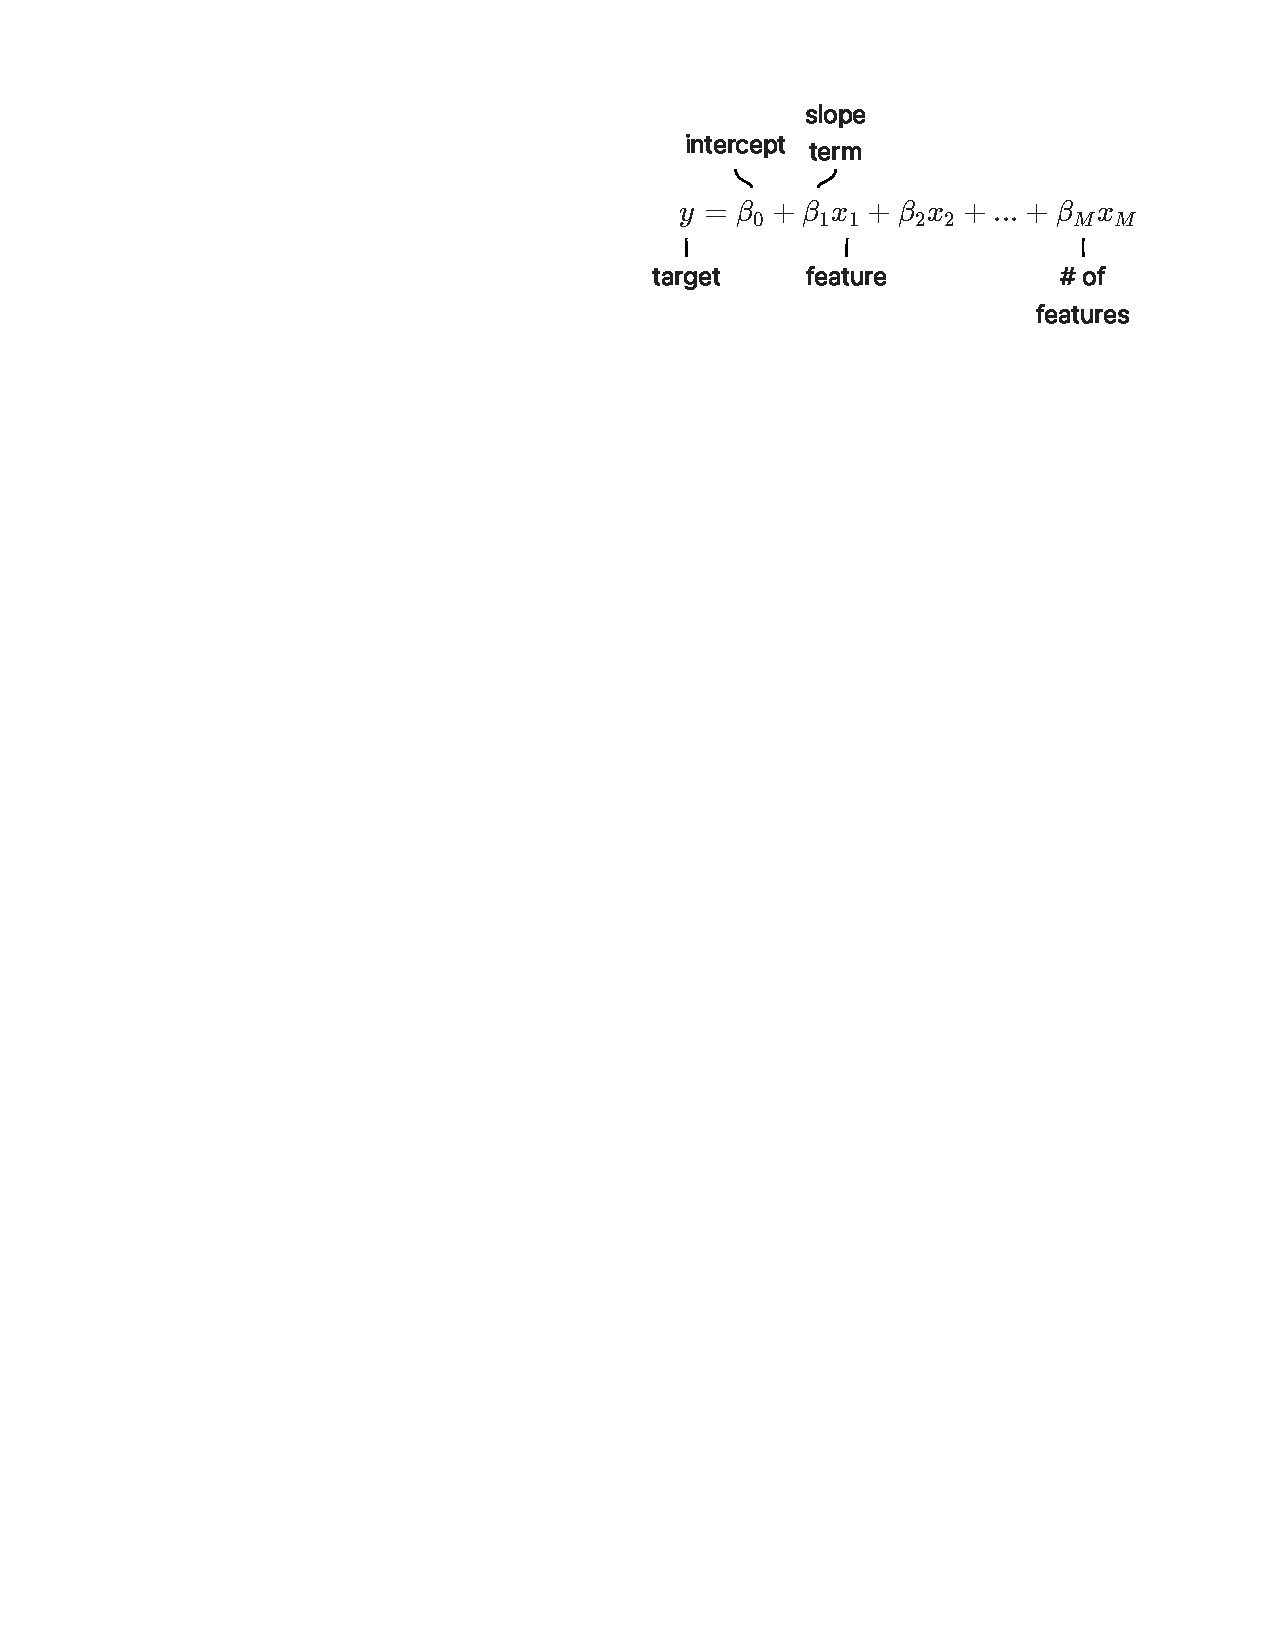
\includegraphics[width=0.65\linewidth]{figures/aug-intro}
\Description{A linear regression formula, augmented with descriptive labels. “y” is labeled “target”; “beta-sub-0” is labeled “intercept”; “beta-sub-1” is labeled “slope term”; “x-sub-1” is labeled “feature”; “beta-sub-M” is labeled “number of features.”}
\vspace{0.5ex}
\end{center}
% \vspace{-.5ex}

This alternative presentation helps a reader to unpack the meaning of a formula. It helps the reader understand the purpose of the formula as predicting a target value from a set of input features. It clarifies that ``$x$'' terms correspond to features, and ``$\beta$'' terms correspond to weights. And it brings the formula into a realm of familiarity by relating ``$\beta_0$'' and ``$\beta_1$'' to the ideas of intercept and slope terms that are taught in algebra class.
Annotated formulas like these help readers grasp their meaning at glance. The annotations' value becomes particularly pronounced when applied to formulas of yet greater complexity and domain specificity.

In this paper, we seek to advance the state of the art in tooling that allows authors to create augmented formulas like these. A recent survey by \citet{ref:head2022math} reveals the challenges present in building effective interactive tooling for this purpose. To start with, conventional formula typesetting tools make it a ``struggle'' to augment formulas. Formula markup gets too messy, and environments provide insufficient support for experimenting with cross-document formula styling choices.

Our contribution is a reinvention of the process of augmenting formulas in typesetting tools. We envision formula augmentation as a process that involves a crisp markup language and live incremental feedback. We reify this vision in \emph{FFL}, or ``Formula Formatting Language,'' a markup language for formula augmentation. FFL is targeted for web-based math document authoring. Its key innovations are a design that splits augmentation markup from formula markup, a CSS-inspired familiar syntax, support for cross-document styling, and an implementation that permits live feedback.

% In this paper, we envision an improved authoring experience where users are enabled to separate their augmentation and formula specifications, apply augmentations to multiple expressions simultaneously, and rapidly experiment with alternative augmentations. The result is a language called \emph{FFL}, or ``Formula Formatting Language,'' and an accompanying live runtime.

% Here, a reader can easily gauge what each variable stands for, track which terms in the equation are related, and understand their usage in the equation.

% While augmentations facilitate better comprehension, the tools that authors use to present formulas often introduce friction in doing so. In a recent survey, \citet{ref:head2022math} describe that authors find themselves using tools that involve clunky markup languages, ugly defaults, and tedious graphic editing.

% One class of tools that poses friction is markup languages for typesetting formulas. Today, TeX~\cite{ref:knuth1986tex} is perhaps the most widely-used markup language for expressing formulas. Yet, augmenting formulas with a TeX tool requires injecting augmentation code (e.g., color and label macros) into the underlying formula. This results in an experience described a ``struggle''~\cite{ref:head2022math} as markup becomes difficult to read and efficiently edit. Furthermore, unless an author has been disciplined about defining expressions using macros, it can be time-consuming to alter style choices across formulas.

% Other challenges of TeX-based environments are that the de facto tool for labeling (i.e., \texttt{mathtools}~\cite{tool:madsen2014mathtools}) introduces unsightly spacing around formulas.

% In this paper, we envision an improved authoring experience where users are enabled to separate their augmentation and formula specifications, apply augmentations to multiple expressions simultaneously, and rapidly experiment with alternative augmentations. The result is a language called \emph{FFL}, or ``Formula Formatting Language,'' and an accompanying live runtime.

% The language and runtime seek to improve the augmentation practice with the following advances. First, FFL is written separately from the LaTeX formula definition to improve readability, similar to how CSS is written separately from HTML, where we draw much of our inspiration. Second, authors use a selector language to identify expressions to augment. This language supports the selection of expressions using LaTeX literals, along with wildcards that allow authors to augment syntactically related expressions (e.g., all symbols $x_*$ with any subscript $*$). Third, FFL supports rapid experimentation by providing a runtime API that integrates with the web-based LaTeX formula typesetting library \textit{KaTeX}~\cite{tool:katex}. Changes to FFL trigger an instant re-rendering of the formula's augmentation. These aspects of FFL aim to support an enhanced augmentation experience with maintainable markup.

% \andrew{Probably we should mention the space of augmentations that the current implementation supports---in particular, color, labeling, and background color, with support for padding and borders for individual symbols}

% Our tool is not the first to propose novel web-based markup formats for augmenting notation---Nota~\cite{ref:crichton2021new} and Heartdown~\cite{ref:li2022heartdown} are two recent examples of markup languages with integrated augmentation features. Where the vision of FFL diverges is in considering augmentation as a styling action similar to what is done with CSS—to develop a selector language support application of augmentations to multiple expressions; and in its development as a technology that could be plugged into arbitrary authoring environments that use KaTeX to typeset formulas. What is more, we also explore the advantages of such augmentation languages in a controlled usability study.

We assess FFL's impact on the authoring experience in a controlled usability study where 28 participants used FFL and \zed{a} LaTeX baseline.
\zed{In complex editing tasks, FFL increased efficiency, self-reported ease, and led to more readable augmentation code versus the baseline. For tasks involving writing simple augmentations from scratch, FFL and LaTeX saw no significant differences.}
% \zed{FFL increased efficiency, self-reported ease, and led to more readable augmentation code when participants performed complex editing tasks, and yielded no observed performance difference for simpler authoring tasks.}
Reviewing the evidence in the framework of the cognitive dimensions of notation~\cite{ref:blackwell2003notational}, our study suggests FFL reduces viscosity, hard mental operations, and error proneness, while benefiting from closeness of mapping and progressive evaluation. These results suggest that FFL-like languages could make the formula augmentation task better supported in contemporary authoring tools.

% We assessed FFL's ability to assist in augmenting formulas in a controlled usability study. In this study, 28 participants used both FFL and LaTeX to author and edit augmentations. The study revealed that, following an initial learning curve, FFL reduced the time to augment formulas and edit augmentations compared to a LaTeX baseline toolset. Furthermore, FFL reduced difficulty and led to more readable augmentation code according to participants' self-reports. In the results, we highlight evidence that, in the parlance of cognitive dimensions of notation~\cite{ref:blackwell2003notational}, FFL reduces viscosity, error proneness, and diffuseness, while increasing the closeness of mapping and supporting progressive evaluation. Our study clarifies what from FFL was found to be valuable to participants, and directions in which languages and runtimes like FFL should evolve to provide an even better utility for authors.
% One additional cognitive dimension I think we support is to reduce premature commitment, but I don't know if we have any evidence supporting that.
% The tasks in authoring that FFL supports include incrementation, modification, exploratory design, and exploratory understanding.

In summary, this paper contributes:
\begin{itemize}
% \vspace{-1ex}
\item The design of \emph{FFL}, a markup language for augmenting formulas, designed for readability and efficiency.
% \item The design of \emph{FFL}, a markup language for augmenting formulas that allows for applying augmentations to classes of expressions within and across formulas.

\item A runtime supporting live application of augmentations to formulas in web-based authoring environments.

% \item A live runtime that integrates with the KaTeX formula typesetting package and supports live application of styles specified in FFL to formulas.

% in web authoring environments that can be triggered by edits to FFL specifications.

\item Evidence from a usability study that FFL leads to faster and easier edits to augmentation markup, and results in more readable markup.
% \vspace{-1ex}
% \item Evidence from a usability study that FFL can be used to edit augmentation code more efficiently and improve the readability of markup, compared to baseline LaTeX tools. 

\end{itemize}

% Old version of the introduction follows.
% Notation is sometimes augmented to make it easier to understand.
% For instance, an author might colorize it in a way that relates expressions in that formula to descriptive passages in nearby text.
% Or, they might write labels for expressions in the margin of the formula.

% Augmenting notation in this way is difficult.
% Key sources of difficulty include the need to open other applications to author augmentations, and the difficulty of reading and writing markup for augmentation.

% What would it take to have robust language support for augmenting formulas? That is the topic of this paper. We posit that robust support for augmenting formulas involves:

% 1. Live application of styles and augmentations
% 2. An easy-to-read, easy-to-write specification language (assuming a markup setting)

% Our vision of specification languages works towards making writing easy in a few ways. First, the language is familiar, extending CSS. Second, the language separates out the content markup for a formula from its presentation markup, keeping the LaTeX for the original formula as readable as it originally was, and avoiding editing issues arising from curly brace nesting. Third, a single augmentation can apply to multiple expressions. Fourth, an augmentation can be written in a way that makes it resilient to changes in the formula (e.g., if a subscript changes).

% Because of its resemblance to CSS, we call the language FFL, for ``Formula Formatting Language.'' The idea of FFL is to separate out the presentation markup; and to declare styles that apply across the page, rather than to individual elements. Our implementation in fact compiles down to CSS (requiring some annotation of the generated HTML for a formula), and thus leverages CSS properties like padding and text color by the nature of its implementation.

% \andrew{The current approach was designed for feasibility of integration, and as such it performs augmentations as an extension to an existing toolkit, having access to nothing but an API that provides access to the tokens in LaTeX strings. This approach works for a broad variety of patterns for colorization, labels, and other styles---we detail the strengths and limitations in the system section.}

% We demonstrate the power of FFL by replicating a number of augmentations that were documented in a recent qualitative study~\cite{ref:head2022math}, and then by conducting a first-use study comparing FFL to the baseline of contemporary typesetting tools.

% FFL is a lightweight language for augmenting formulas that has been designed to be concise, readable, and writable. We develop an accompanying runtime that augments typeset formulas live in web authoring environments as an author writes FFL. The language and runtime together were developed with the aim of supporting an augmentation experience where markup is easy to read and write, authors receive rapid feedback, augmentations like labels are aesthetically pleasing by default, and augmentations can be applied quickly across multiple expressions in one or more formulas.

% FFL offers several innovations choices that lead to this experience are three-fold. First,  FFL provides a selector language that allows authors to apply augmentations to groups of expressions, rather than individual expressions. 

% how markup tools could be redesigned to support clean, efficient augmentation of formulas

% This research was motivated by a feeling that new syntaxes were needed that could provide both a low threshold and eventually a high ceiling~\cite{ref:myers2000past}, along with simple expression of common augmentations. For instance, we believe it should be easy to colorize formulas, and to define always-on augmentation; these require a different way of thinking about processing the markup. Furthermore, we envision leveraging authors' existing knowledge of languages like CSS to support their writing.